\documentclass[tikz, border=10pt]{standalone}

\usepackage{tikz}
\usetikzlibrary{snakes}

% define styles
\tikzset{
    wave/.style = {snake=coil, segment length=2mm, segment amplitude=2mm, segment aspect=0, line before snake=0.5mm, line after snake=1mm},
    interface/.style = {snake=border, segment angle=-45, segment length=2mm, segment amplitude=3mm},
    medium/.style = {font={\footnotesize\sffamily}}
}

\begin{document}
    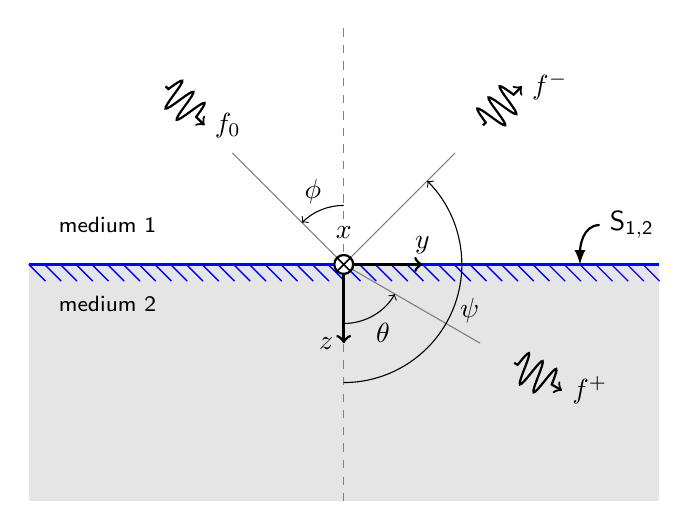
\begin{tikzpicture}
        % draw gray rectangle
        \fill[gray!20] (-4, -3) rectangle (4, 0);
        % draw blue line and its border pattern
        \draw[thick, blue] (-4, 0) -- (4, 0);
        \draw[interface, line width=0.5pt, blue] (-4, 0) -- (4, 0);
        % draw vertical dashed line
        \draw[dashed, gray] (0, 3) -- (0, 0) node[above=2mm, black] {$x$} -- (0, -3);
        % draw coordinate system
        \draw[<->, line width=1pt] (1, 0) node[above] {$y$} -| (0, -1) node[left] {$z$};
        % incidence
        \draw[gray] (0, 0) -- +(135:2);
        \draw[->] (90:0.75) arc (90:135:0.75);
        \draw (113:1) node {$\phi$};
        \draw[->, wave, thick] (135:3.2) -- (135:2.5) node[right] {$f_0$};
        % transmission
        \draw[gray] (0, 0) -- +(45:2);
        \draw[gray] (0, 0) -- +(-30:2);
        \draw[->] (-90:0.75) arc (-90:-30:0.75);
        \draw (0, 0) +(-60:1) node {$\theta$};
        \draw[->, wave, thick] (-30:2.5) -- (-30:3.2) node[right] {$f^{+}$};
        % reflection
        \draw[->] (0, 0) +(-90:1.5) arc (-90:45:1.5);
        \node at (-20:1.7) {$\psi$};
        \draw[->, wave, thick] (45:2.5) -- (45:3.2) node[right] {$f^{-}$};
        % interface pointer
        \draw[-latex, thick] (3.25, 0.5) node[right] {$\mathsf{S_{1, 2}}$} to[out=180, in=90] (3, 0);
        % x axis
        \filldraw[fill=white, thick] (0, 0) circle (0.12cm);
        \draw[line width=0.6pt] (135:0.12) -- (-45:0.12)
                                (45:0.12) -- (-135:0.12);
        % medium names
        \draw (-3, 0.5) node[medium] {medium 1};
        \draw (-3, -0.5) node[medium] {medium 2};
    \end{tikzpicture}
\end{document}